% =====================================================================
%  TFM - Master en Machine Learning for Health (UC3M)
%  Portada oficial UC3M + cuerpo en formato IEEE (IEEEtran, 2 columnas)
%  Bibliografia con BibTeX -> referencias.bib
% =====================================================================
\documentclass[10pt,conference]{IEEEtran}

% --- Idioma y codificacion ------------------------------------------
\usepackage[utf8]{inputenc}
\usepackage[T1]{fontenc}
\usepackage[english]{babel}

% --- Matematicas ----------------------------------------------------
\usepackage{amsmath,amssymb,amsfonts}

% --- Graficos, color, tablas ----------------------------------------
\usepackage{graphicx}
\usepackage{float}
\graphicspath{{imagenes/}}
\usepackage[table]{xcolor}
\definecolor{azulUC3M}{RGB}{0,0,102}
\usepackage{booktabs}
\usepackage{multirow}
\usepackage{tabularx}
\usepackage{subcaption}

% --- Unidades y algoritmos ------------------------------------------
\usepackage{siunitx}
\sisetup{
  detect-all,
  range-units          = single,
  separate-uncertainty = true,
  per-mode             = symbol
}
\usepackage{algorithm}
\usepackage{algpseudocode}

% --- Citas IEEE + enlaces (hyperref SIEMPRE el ultimo) --------------
\usepackage{cite}
\usepackage[hidelinks]{hyperref}

% --- Numeracion de pagina centrada al pie ---------------------------
\makeatletter
\def\ps@tfmplain{%
  \let\@oddhead\@empty\let\@evenhead\@empty
  \def\@oddfoot{\hfil\thepage\hfil}\let\@evenfoot\@oddfoot
}
\let\ps@IEEEtitlepagestyle\ps@tfmplain
\makeatother


\begin{document}

% =====================================================================
% 1) PORTADA OFICIAL UC3M
% =====================================================================
\begin{titlepage}
\begin{sffamily}
\color{azulUC3M}
\begin{center}

  \begin{figure}[H]
    \makebox[\textwidth][c]{
\includegraphics[width=16cm]{logo_UC3M.png}}
  \end{figure}

  \vspace{2.5cm}
  \begin{Large}
    Master Degree in Machine Learning for Health\\
    2025-2026\\
    \vspace{2cm}
    \textsl{Master Thesis}
    \bigskip
  \end{Large}

  {\Huge ``Deep Learning for Photomultiplier Crystal Detection Signals''}\\
  \vspace*{0.5cm}
  \rule{10.5cm}{0.1mm}\\
  \vspace*{0.9cm}

  {\LARGE Miguel Escudero Rodr\'iguez}\\
  \vspace*{1cm}

  \begin{Large}
    David Izquierdo-Garc\'ia\\
    Legan\'es, September 2026\\
  \end{Large}

\end{center}
\vfill
\color{black}

\fbox{%
\begin{minipage}{\linewidth}
  \textbf{AVOID PLAGIARISM}\\
  \footnotesize{The University uses the \textbf{Turnitin Feedback Studio} for the
  delivery of student work. This program compares the originality of the work
  delivered by each student with millions of electronic resources and detects
  those parts of the text that are copied and pasted. Plagiarizing in a TFM is
  considered a \textbf{\underline{Serious Misconduct}}, and may result in
  permanent expulsion from the University.}
\end{minipage}}

\vspace{0.5cm}
\noindent
\includegraphics[width=4.2cm]{creativecommons.png}\\
\footnotesize{This work is licensed under Creative Commons
\textbf{Attribution -- Non Commercial -- Non Derivatives}}

\end{sffamily}
\end{titlepage}

\setcounter{page}{1}


% =====================================================================
% 2) CUERPO
% =====================================================================

\title{Deep Learning for Photomultiplier Crystal Detection Signals}

\author{%
\IEEEauthorblockN{Miguel Escudero Rodr\'iguez}
\IEEEauthorblockA{%
Master's Degree in Machine Learning for Health\\
Universidad Carlos III de Madrid, Legan\'es, Spain\\
Email: 100569281@alumnos.uc3m.es}
}

\maketitle
\pagestyle{tfmplain}

\begin{abstract}
TODO: 150--250 palabras. Problema, metodo propuesto, datos empleados y
resultados cuantitativos principales.
Lorem ipsum dolor sit amet, consectetur adipiscing elit. Sed do eiusmod tempor incididunt ut labore et dolore magna aliqua. Ut enim ad minim veniam, quis nostrud exercitation ullamco laboris nisi ut aliquip ex ea commodo consequat. Duis aute irure dolor in reprehenderit in voluptate velit esse cillum dolore eu fugiat nulla pariatur. Excepteur sint occaecat cupidatat non proident, sunt in culpa qui officia deserunt mollit anim id est laborum.

Curabitur pretium tincidunt lacus. Nulla gravida orci a odio, sed fermentum lorem interdum. Phasellus convallis, sapien nec facilisis tincidunt, justo lectus malesuada erat, vitae consectetur neque arcu vel lorem. Integer consequat, augue a interdum consequat, erat sapien volutpat justo, at tincidunt libero mauris nec nisl. Vestibulum ante ipsum primis in faucibus orci luctus et ultrices posuere cubilia curae; Donec vitae augue sed justo interdum tincidunt.

Mauris euismod, lectus vitae tincidunt posuere, justo sem malesuada neque, eget feugiat sapien nisl a erat. Aenean interdum, purus vel malesuada consequat, magna sapien tincidunt augue, non consequat libero neque at justo. Suspendisse potenti. Proin vitae lorem at ipsum interdum tincidunt. Aliquam erat volutpat. Nam sed augue vel risus commodo interdum, sed tincidunt justo consequat. Pellentesque habitant morbi tristique senectus et netus et malesuada fames ac turpis egestas. Integer vel lorem nec sapien facilisis aliquam. Donec vulputate, magna at consequat suscipit, justo neque malesuada nisl, vitae tincidunt erat turpis vel ipsum. Vivamus feugiat lorem sed arcu malesuada, quis consequat purus tincidunt. Sed euismod, neque vitae interdum consequat, justo sapien fermentum mauris, vel tincidunt nulla nisl non erat.

\end{abstract}

\begin{IEEEkeywords}
Positron emission tomography, silicon photomultiplier, missing data
imputation, deep learning, detector calibration.
\end{IEEEkeywords}


% ---------------------------------------------------------------------
\section{Introduction}
% ---------------------------------------------------------------------


Positron Emission Tomography (PET) is a non-invasive molecular imaging
modality and one of the central techniques of nuclear medicine, providing
an \textit{in vivo} assessment of the metabolic and biochemical state of a
patient \cite{cherry2012}. Unlike purely anatomical modalities, PET relies
on radiotracers: biologically active molecules chemically labelled with
positron-emitting radionuclides \cite{rong2023}. Once administered, the
tracer distributes according to the physiological pathway targeted by its
carrier molecule, so that the measured signal reflects function rather than
structure. When an emitted positron annihilates with an electron in the
surrounding tissue, two photons of 511\,keV --- the rest mass energy of the
electron --- are released in nearly opposite directions. Detecting both of
them in coincidence defines a line of response (LOR) along which the
annihilation took place, and the accumulation of millions of LORs allows the
three-dimensional distribution of activity to be reconstructed
\cite{cherry2012}. This detection scheme gives PET a functional sensitivity that few other non-invasive imaging techniques can match \cite{vaquero2015}, at the
price of the tracer itself: positron-emitting radionuclides are radioactive
by nature, costly to produce, and short-lived, which ties any PET facility
to a nearby cyclotron and specific facilities \cite{rong2023}.

This functional readout is most valuable where disease alters metabolism
before it alters anatomy. In oncology, $^{18}$F-FDG PET has become a
cornerstone for diagnosis, staging, restaging and the assessment of
treatment response \cite{fletcher2008,boellaard2015}. Its role in neurology
is arguably even more distinctive, since it reveals pathologies that produce
no macroscopic structural abnormality on conventional Magnetic Resonance
Imaging (MRI) or Computed Tomography (CT), such as the characteristic
hypometabolic and amyloid patterns of Alzheimer's disease
\cite{johnson2013}, among other neurodegenerative and cerebrovascular
disorders.

The sensitivity of PET is not matched by its spatial resolution. Clinical
scanners typically resolve 4--5\,mm FWHM \cite{spencer2021}, and
recent advances push the number towards 3\,mm \cite{spencer2021,
gonzalezmontoro2022brain} , higher than the numbers normally achieved with MRI or CT. This limit decomposes into four
contributions, two physical and two belonging to the detector, which behave
very differently from one another \cite{moses2011}. The physical ones are
the finite distance the positron travels before annihilating, set by the
emitting isotope \cite{levin1999}, and the small angular deviation from
antiparallel emission, caused by the residual momentum of the
electron--positron pair. Neither can be engineered away, although the second
translates into a positional error that scales with the diameter of the
detector ring and is therefore smaller in compact systems. The detector terms are more tractable. In pixelated arrays, the size of the
individual element fixes the finest scale at which an interaction can be
localised; shrinking it improves resolution, but the inter-crystal
reflectors then occupy a growing fraction of the detector volume, and the
probability that a photon deposits energy across several elements rises.
The decoding error --- the uncertainty in determining where within the
module the interaction occurred --- amounts to roughly one third of the
detector width \cite{moses2011}. Unlike positron range and non-collinearity,
this term is not a physical floor but a consequence of how the light
distribution is read and interpreted, and it is therefore the one most open to improvement, whether through detector geometry, readout electronics or the algorithms that interpret
the signal.
This is the ground occupied by organ-dedicated scanners. Adapting the
detector geometry to a specific anatomical region increases solid-angle
coverage, and with it sensitivity and resolution, at a lower manufacturing
cost than a general-purpose whole-body system; designs exist for breast,
brain, prostate and cardiac imaging \cite{sanaat2024}. The trade-off is that
irregular geometries complicate calibration and data correction, and that
small gantry apertures accentuate parallax errors and degrade the uniformity
of spatial resolution across the field of view \cite{sanaat2024}. Much of
the design effort in these systems therefore shifts onto the detector
itself.

Our group is currently developing a quasi-spherical brain-dedicated PET
scanner along these lines \cite{perez-benito_sipm-based_2019}. Rather than
the cylindrical ring of conventional systems, its detector modules tile a
closed surface around the head (Fig.~\ref{fig:escaner}), approaching full $4\pi$ steradian coverage
and thereby collecting a far larger fraction of the emitted coincidences
\cite{perez-benito_sipm-based_2019}. The modules are hexagonal, a shape
chosen for two independent reasons: hexagons tile a surface without gaps and
approximate a sphere more closely than square modules of comparable size,
and hexagonal scintillators have also been shown to offer slightly better
light yield and energy resolution than square, triangular or cylindrical
prisms \cite{perez-benito_scintillator_2023}.Each module is built around a monolithic LYSO crystal
\cite{perez-benito_laser-microstructured_2025}.

\begin{figure}[t]
\centering
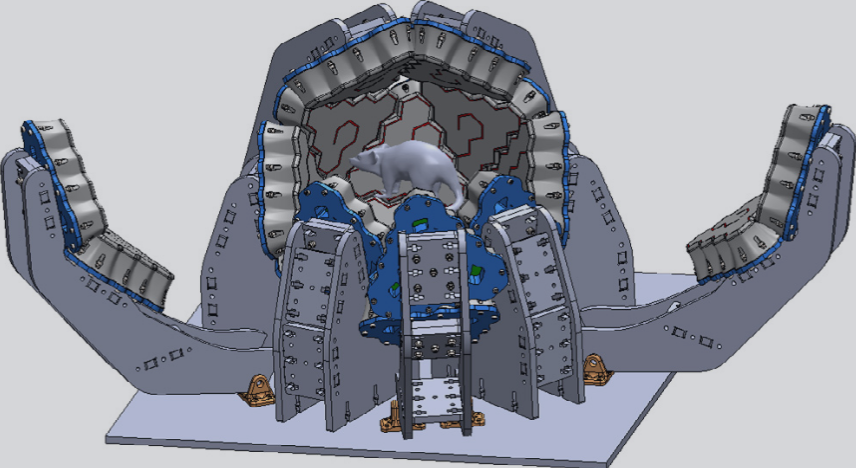
\includegraphics[width=\linewidth]{escaner}
\caption{\textbf{TEMPORAL}Three-dimensional model of the quasi-spherical, hexagonal-based
PET scanner. Reproduced from \cite{perez-benito_sipm-based_2019}.}
\label{fig:escaner}
\end{figure}

The choice between segmenting the scintillator and leaving it continuous is
not incidental, and it conditions how the interaction position can be
recovered at all \cite{gonzalezmontoro2022}. In pixelated arrays, the
crystal is cut into individual elements separated by reflectors, so that the
interaction is assigned to whichever element fired. Event positioning is
then simple and fast, but the resolution cannot be finer than the element
itself \cite{moses2011}, and two costs follow from making the elements
smaller: the reflectors occupy a growing fraction of the detector volume,
reducing the packing fraction, and the number of readout channels rises.
Multiplexing schemes, in which several crystals share a readout line and the
position is recovered by decoding the light distribution, are commonly used
to keep this cost manageable \cite{sanaat2024}. Pixelated arrays also
provide no intrinsic depth-of-interaction information, which has motivated
layered designs such as phoswich detectors, where stacked scintillators with
different decay times allow a coarse depth assignment at the price of a
degraded timing resolution \cite{sanaat2024}.

Monolithic scintillators take the opposite approach. A single continuous
block is coupled to an array of photodetectors, and the light from each
interaction spreads over many channels at once \cite{gonzalezmontoro2022}. 
Positioning is no longer a matter of identifying an element but of
estimating a coordinate from the recorded light distribution, which shifts
the resolution limit from the geometry of the crystal to the quality of the
positioning algorithm, and makes the depth of interaction recoverable as a
continuous variable \cite{espana_digipet_2014}. The absence of internal reflectors
also restores the packing fraction lost in segmented designs
\cite{sanaat2024}. This is the configuration adopted in the scanner
described above, and it is the one this work builds on.


\begin{figure}[t]
\centering
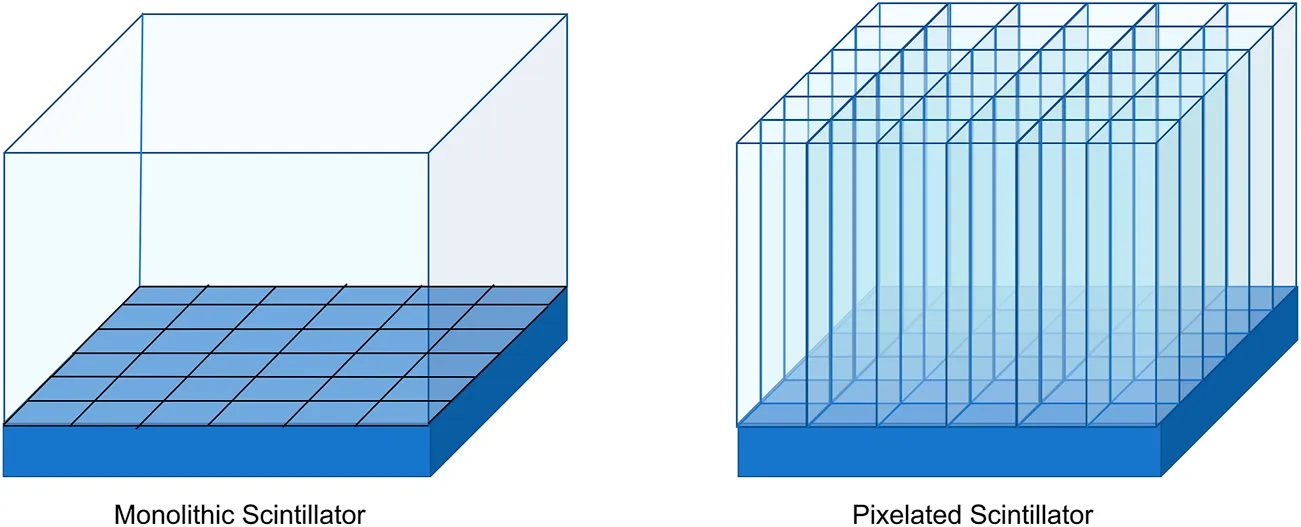
\includegraphics[width=\linewidth]{cristales}
\caption{Monolithic (left) versus pixelated (right) scintillator
configurations. In the monolithic design a continuous slab is coupled to a
segmented photosensor array; in the pixelated design the crystal is cut into
elements coupled one-to-one to the photosensors. Reproduced from
\cite{enlow2023} under CC BY 4.0.}
\label{fig:cristales}
\end{figure}


% ---------------------------------------------------------------------
\section{Materials and Methods}
% ---------------------------------------------------------------------

\subsection{Detector Module}
\label{sec:detector}

Every measurement in this work comes from a single detector module of the
scanner described above. The scintillator is a monolithic LYSO hexagonal
prism, 17.6\,mm on a side and 13\,mm thick, laser-etched into 364
honeycomb-like optical structures that constrain how the scintillation light
spreads before it reaches the photosensor
\cite{perez-benito_laser-microstructured_2025}. The back face is optically
coupled to an array of silicon photomultipliers
\cite{perez-benito_sipm-based_2019}, whose individual cells convert the light
into a charge $R_{ch}$ read out per channel \cite{gundacker2020}. The lateral
faces carry an absorbing black adhesive that suppresses edge reflections; as a
side effect, interactions near the perimeter lose a measurable fraction of
their scintillation light, which is visible later in both the per-channel
charge and the energy spectrum.
% TODO(dato): modelo concreto de SiPM y dimensiones de la celda activa.

The array provides 64 readout channels, of which 61 are instrumented in the
module used here; channels 1, 16 and 18 are inactive and we excluded them
throughout. Table~\ref{tab:detector} lists the geometry we derived directly
from the physical sensor positions. The 61 active centres tile a hexagonal
lattice of side 5 with a pitch of 3.75\,mm, spanning
$[-13.0, 13.0]$\,mm in $x$ and $[-15.0, 15.0]$\,mm in $y$. The ratio between
these two half-extents, $13/15 = 0.867$, matches $\cos 30^{\circ}$ to three
decimal places, confirming a regular hexagonal envelope with vertices along
$y$. The sensor centres therefore do not reach the crystal boundary, which is
consistent with the larger crystal side quoted above.

\begin{table}[t]
\centering
\caption{Geometry of the detector module, obtained from the physical sensor
positions.}
\label{tab:detector}
\begin{tabular}{@{}lc@{}}
\toprule
\textbf{Property} & \textbf{Value} \\
\midrule
Crystal                       & Monolithic LYSO, hexagonal \\
Crystal side / thickness      & 17.6\,mm / 13\,mm \\
Etched optical structures     & 364 \\
Total readout channels        & 64 \\
Instrumented channels         & 61 \\
Inactive channels ($\mathrm{Ich}$) & 1, 16, 18 \\
Sensor pitch                  & 3.75\,mm \\
Extent in $x$                 & $[-13.0,\ 13.0]$\,mm \\
Extent in $y$                 & $[-15.0,\ 15.0]$\,mm \\
Maximum radius from centre    & 15.01\,mm \\
Lattice                       & Hexagonal, side 5 \\
\bottomrule
\end{tabular}
\end{table}

A 511\,keV gamma interacting in the crystal releases on the order of
$10^{4}$ optical photons, which distribute over many channels at once. We
estimated the interaction position with an Anger-type centroid weighted by the
squared charge,
%
\begin{equation}
\hat{x} = \frac{\sum_{c} R_{ch,c}^{2}\, x_{c}}{\sum_{c} R_{ch,c}^{2}},
\qquad
\hat{y} = \frac{\sum_{c} R_{ch,c}^{2}\, y_{c}}{\sum_{c} R_{ch,c}^{2}},
\label{eq:centroid}
\end{equation}
%
where $(x_{c}, y_{c})$ are the sensor coordinates. The two-dimensional
histogram of $(\hat{x}, \hat{y})$ over many events is the flood map, and it is
the image in which the 364 structures must remain separable.

\subsection{Dataset}
\label{sec:dataset}

We used acquisitions recorded with a $^{22}$Na source, one binary file per
physical detector module. The collection comprises 159 nominally healthy
modules, referred to as \textsc{Good}, and 62 modules with at least one
suspected faulty channel, referred to as \textsc{Bad}. Each file holds on the
order of $10^{6}$ events and occupies about 161\,MB, for a total of 25.5\,GB in
the \textsc{Good} set. Table~\ref{tab:dataset} summarises the statistics.
% TODO(dato): actividad de la fuente de 22Na, geometria de irradiacion y
% duracion de cada adquisicion.
% TODO(dato): modelo de ASIC y valor del umbral de discriminacion aplicado.

\begin{table}[t]
\centering
\caption{Dataset statistics. Charges are expressed in ADC units.}
\label{tab:dataset}
\begin{tabular}{@{}lc@{}}
\toprule
\textbf{Property} & \textbf{Value} \\
\midrule
\textsc{Good} modules              & 159 \\
\textsc{Bad} modules               & 62 \\
Mean file size                     & 161\,MB \\
Total volume (\textsc{Good})       & 25.5\,GB \\
Events per file                    & $\sim 10^{6}$ \\
Events in the test partition       & \num{5476642} \\
Active channels per event (mean)   & 17.0 \\
Active channels per event (range)  & 1--54 \\
Total charge $R_T$ (mean)          & 31.9 \\
Total charge $R_T$ (median)        & 26.8 \\
\bottomrule
\end{tabular}
\end{table}

The gap between the mean and the median of $R_T$ reflects the asymmetry of the
energy distribution, with a high-energy tail over a dominant Compton
background. We applied no energy calibration and no energy window, a choice we
return to in Section~\ref{sec:metrics}, where the spectral metric is
constructed so that this omission cancels.

We split the \textsc{Good} set \emph{by file} rather than by event, using a
fixed seed of 42: 149 modules for training, 5 for validation and 5 held out for
testing (\texttt{datas057}, \texttt{116}, \texttt{126}, \texttt{202} and
\texttt{214}). The distinction matters. Each file is a different physical
detector, so splitting by file measures generalisation to hardware the model
has never seen, whereas splitting by event would measure a considerably easier
problem. The test partition was reserved from the outset and used neither for
training nor for model selection.

\subsection{Problem Formulation}
\label{sec:formulation}

Let $\mathbf{r} \in \mathbb{R}^{61}$ be the vector of channel charges for one
event. We modelled a faulty channel by forcing a subset
$\mathcal{D} \subset \{1, \dots, 61\}$ of entries to zero, and asked the model
to recover the original vector from what remains. The masked input is
%
\begin{equation}
\tilde{r}_{c} =
\begin{cases}
0 & \text{if } c \in \mathcal{D} \\
r_{c} & \text{otherwise,}
\end{cases}
\label{eq:mask}
\end{equation}
%
and the network additionally receives the binary mask
$m_{c} = \mathbb{1}[c \notin \mathcal{D}]$, so that a channel switched off is
distinguishable from a channel that legitimately recorded no signal. Input and
target share the same normalising factor, the maximum of the masked vector:
%
\begin{equation}
\mathbf{x} = \frac{\tilde{\mathbf{r}}}{\max_{c} \tilde{r}_{c}},
\qquad
\mathbf{y} = \frac{\mathbf{r}}{\max_{c} \tilde{r}_{c}}.
\label{eq:norm}
\end{equation}
%
Because the normaliser is computed \emph{after} masking, the target of a
suppressed channel may exceed unity when that channel was the brightest of the
event. The network output is therefore linear, with no sigmoid or clamp. We
clipped negative charges to zero before masking, and we normalised per event
rather than per dataset: for position estimation what matters is how the light
distributes, not how much light there was in total.

This construction is a masked autoencoder \cite{he2022mae} applied to detector
channels instead of image patches, and it makes the task self-supervised. The
ground truth is the original 61-channel vector, so no module with a genuinely
dead sensor is needed for training, and the supervision requires no
calibration. We generated the masks on the fly, drawing a fresh $\mathcal{D}$
for every sample, so a given event is never seen twice with the same failure
pattern.

Two aspects of the sampling deserve mention. The first is class balance: half
of the samples suppress a channel that did carry signal and half suppress a
channel already at zero. Without this balance roughly three quarters of the
examples would require no correction at all, and the model would reasonably
learn to do nothing.

The second is the spatial pattern of $\mathcal{D}$, which we controlled through
three regimes. In \emph{cluster} the $k$ suppressed channels are contiguous; in
\emph{scatter} they are drawn uniformly across the detector; and in \emph{near}
they lie within two hops of the seed without being required to touch. The
motivation for the third regime is empirical. When we labelled the \textsc{Bad}
modules, the failures we found most often were neither compact groups nor
sensors scattered across the whole array, but two or three sensors separated by
one or two positions.

\subsection{Architectures}
\label{sec:architectures}

We evaluated four families of models, all solving the same $61 \rightarrow 61$
regression.

\subsubsection{Classical baselines}
Two methods without learned parameters establish what the geometry alone
provides: the mean of the neighbouring channels, and a linear regression fitted
per channel on the remaining 60. Both exclude the target channel from their
inputs, and we fitted the regression coefficients on training modules only.

\subsubsection{Baselines without a geometric prior}
A deep multilayer perceptron (\textsc{DeepMLP}) and a residual MLP with
attention (\textsc{ResidualMLP}) take the 61 channels as a flat vector. They
have access to the same information but no notion of which sensors are adjacent,
which isolates the contribution of the geometric prior.

\subsubsection{HexGNN}
Our reference model treats the detector as a graph whose 61 nodes are the
active sensors and whose edges join physically adjacent ones. The adjacency
follows the hexagonal lattice: 312 directed edges, with 37 nodes of degree 6,
18 of degree 4 and 6 of degree 3, and full symmetry. Each layer updates a node
from its own state and the mean of its neighbours,
%
\begin{equation}
h_{c}^{(l+1)} = \sigma\!\left( W_{s} h_{c}^{(l)}
  + W_{n} \frac{1}{|\mathcal{N}(c)|} \sum_{j \in \mathcal{N}(c)} h_{j}^{(l)}
  + b \right),
\label{eq:hexconv}
\end{equation}
%
with $\sigma$ a GELU nonlinearity. The aggregation is isotropic: all neighbours
of a node share the weight matrix $W_{n}$. The reference configuration
(\textsc{HexGNN-s}) uses a hidden width of 48 and four blocks, for
\num{38305} trainable parameters. We also trained wider variants,
\textsc{HexGNN-m} and \textsc{HexGNN-l}, to test whether capacity was the
binding constraint.

\subsubsection{Architectural variants}
On top of the reference we explored nine modifications, each targeting a
specific hypothesis: metric edge features (relative distances and vectors),
anisotropic hexagonal convolution with one weight per direction, global
attention and a graph transformer, an encoder--decoder with a latent
bottleneck, multi-statistic aggregation, per-channel equalisation,
heteroscedastic prediction of mean and variance, and averaging ensembles.

\subsection{Loss Function}
\label{sec:loss}

We computed the loss over the full 61-channel output rather than the suppressed
entries alone, treating the task as ordinary regression. Our reference is the
mean squared error,
%
\begin{equation}
\mathcal{L} = \frac{1}{61} \sum_{c=1}^{61} \left( \hat{y}_{c} - y_{c} \right)^{2},
\label{eq:loss}
\end{equation}
%
selected after comparing it against the mean absolute error and the Huber loss
with $\delta = 0.1$. We additionally tested two physics-informed terms, one
penalising the position error of Eq.~\ref{eq:centroid} and one penalising the
shift of the energy spectrum, both reported in Section~\ref{sec:results}.

\subsection{Training Setup}
\label{sec:training}

Table~\ref{tab:hyperparams} lists the configuration. One aspect of the schedule
requires clarification, because the word ``epoch'' does not carry its usual
meaning here: each epoch loads \emph{one} detector module and draws
\num{107000} events from it. The 149 epochs therefore correspond to the 149
training modules, each visited once, and the number is set by the partition
rather than tuned. The resulting budget of \num{15943000} samples matches the
one used before full coverage was adopted, so that changes in coverage are not
confounded with changes in cost.

We trained with AdamW and a cosine schedule whose period equals the number of
epochs. We applied no early stopping, since every epoch supplies previously
unseen data, and we selected the final checkpoint by the validation error on
the imputed channel, computed on a fixed set of \num{400000} events with a
fixed mask seed. Every run stores its preprocessing configuration inside the
checkpoint, so that an evaluation cannot silently apply a normalisation
different from the one used in training.

\begin{table}[t]
\centering
\caption{Training configuration of the reference model.}
\label{tab:hyperparams}
\begin{tabular}{@{}lc@{}}
\toprule
\textbf{Property} & \textbf{Value} \\
\midrule
Modules per epoch          & 1 \\
Epochs (= training modules) & 149 \\
Events per epoch           & \num{107000} \\
Total sample budget        & \num{15943000} \\
Batch size                 & 512 \\
Optimiser                  & AdamW \\
Learning rate              & $10^{-3}$ \\
Weight decay               & $10^{-4}$ \\
Scheduler                  & Cosine, $T_{\max} = 149$ \\
Early stopping             & None \\
Checkpoint selection       & Validation MAE, imputed channel \\
Validation events          & \num{400000} \\
Loss                       & MSE \\
\bottomrule
\end{tabular}
\end{table}

\subsection{Evaluation Metrics}
\label{sec:metrics}

The quantity we ultimately care about is not the charge of the recovered
channel but the position it yields, so our primary metric is defined on
Eq.~\ref{eq:centroid}. For each event we computed the displacement $\Delta R$
between the true centroid and the centroid obtained after suppressing a
channel, both without correction (\emph{degraded}) and after imputation
(\emph{imputed}). The recovery is the fraction of that displacement which the
model removes,
%
\begin{equation}
\mathrm{Recovery} = 100 \times
  \left( 1 - \frac{\Delta R_{\text{imp}}}{\Delta R_{\text{deg}}} \right),
\label{eq:recovery}
\end{equation}
%
where numerator and denominator are evaluated at the same quantile and over the
same population of events. We report the value at the 90th percentile, which
weights the difficult events, and we also report the mean. Averaging over the
61 channels gives the macro figures used throughout
Section~\ref{sec:results}, and the minimum over channels characterises the
worst case.

As secondary metrics we used the mean absolute error on the imputed channel in
normalised units, the bias as a guardrail against systematic under-prediction,
and the relative charge error. Two additional analyses address physical
fidelity rather than accuracy. The first measures the point-spread function of
the flood map, comparing its FWHM before and after imputation. The second
measures the preservation of the energy spectrum by zones of the crystal,
defined through concentric hexagonal bands, using a paired differential design:
we subtract the true channel and add back the prediction over the same events,
so that the absence of energy calibration cancels between the two terms.

Finally, to evaluate the pipeline on genuinely faulty hardware, we used a
position-aware statistic that flags anomalous channels in the \textsc{Bad}
modules from the robust $z$-score of two quantities, the fraction of events in
which a channel fires and its charge ratio against its neighbours, both
referenced to the baseline built from the \textsc{Good} modules. This addresses
the same task that industrial practice solves by masking the affected channel
and compensating downstream \cite{philips2015deadpixel}.


% ---------------------------------------------------------------------
\section{Results}
\label{sec:results}
% ---------------------------------------------------------------------

\subsection{Value of the Geometric Prior}

Table~\ref{tab:architectures} compares the architectures under a common
evaluation campaign of \num{600000} events per test file. The two models
without a geometric prior reach 51.39\,\% and 48.92\,\% recovery at the 90th
percentile, while the smallest graph model reaches 58.02\,\% with an order of
magnitude fewer parameters. Widening the graph model, however, changes little: 58.27\,\% for
\textsc{HexGNN-m} and 57.47\,\% for \textsc{HexGNN-l}, against 58.02\,\% for
the 38\,k-parameter reference.

\begin{table}[t]
\centering
\caption{Architecture comparison. Common campaign of \num{600000} events per
test file. Recovery in per cent, MAE in normalised units.}
\label{tab:architectures}
\begin{tabular}{@{}lrccc@{}}
\toprule
\textbf{Model} & \textbf{Params} & \textbf{Rec.\ p90} & \textbf{Rec.\ mean} & \textbf{MAE} \\
\midrule
DeepMLP          & \num{500541}  & 51.39 & 45.90 & 0.7219 \\
ResidualMLP      & \num{345981}  & 48.92 & 44.81 & 0.7299 \\
Graphormer       & \num{4263881} & 55.17 & 49.65 & 0.6600 \\
Graph U-Net      & \num{331649}  & 55.22 & 47.95 & 0.6918 \\
PNA              & \num{165761}  & 58.45 & 52.48 & 0.6309 \\
\textsc{HexGNN-s} & \num{38305}  & 58.02 & 52.66 & 0.6195 \\
\textsc{HexGNN-m} & \num{225217} & 58.27 & 52.64 & 0.6185 \\
\textsc{HexGNN-l} & \num{398593} & 57.47 & 51.96 & 0.6385 \\
\bottomrule
\end{tabular}
\end{table}

To test whether the graph structure itself carries the advantage, rather than
the inductive bias of message passing in general, we retrained the reference
with the adjacency randomly permuted, preserving the number of nodes, the
number of edges and the degree distribution. Recovery falls to 28.08\,\%,
27.66\,\% and 31.28\,\% across three shuffles (Fig.~\ref{fig:ablacion}),
against 58.02\,\% for the true adjacency.

\begin{figure}[t]
\centering
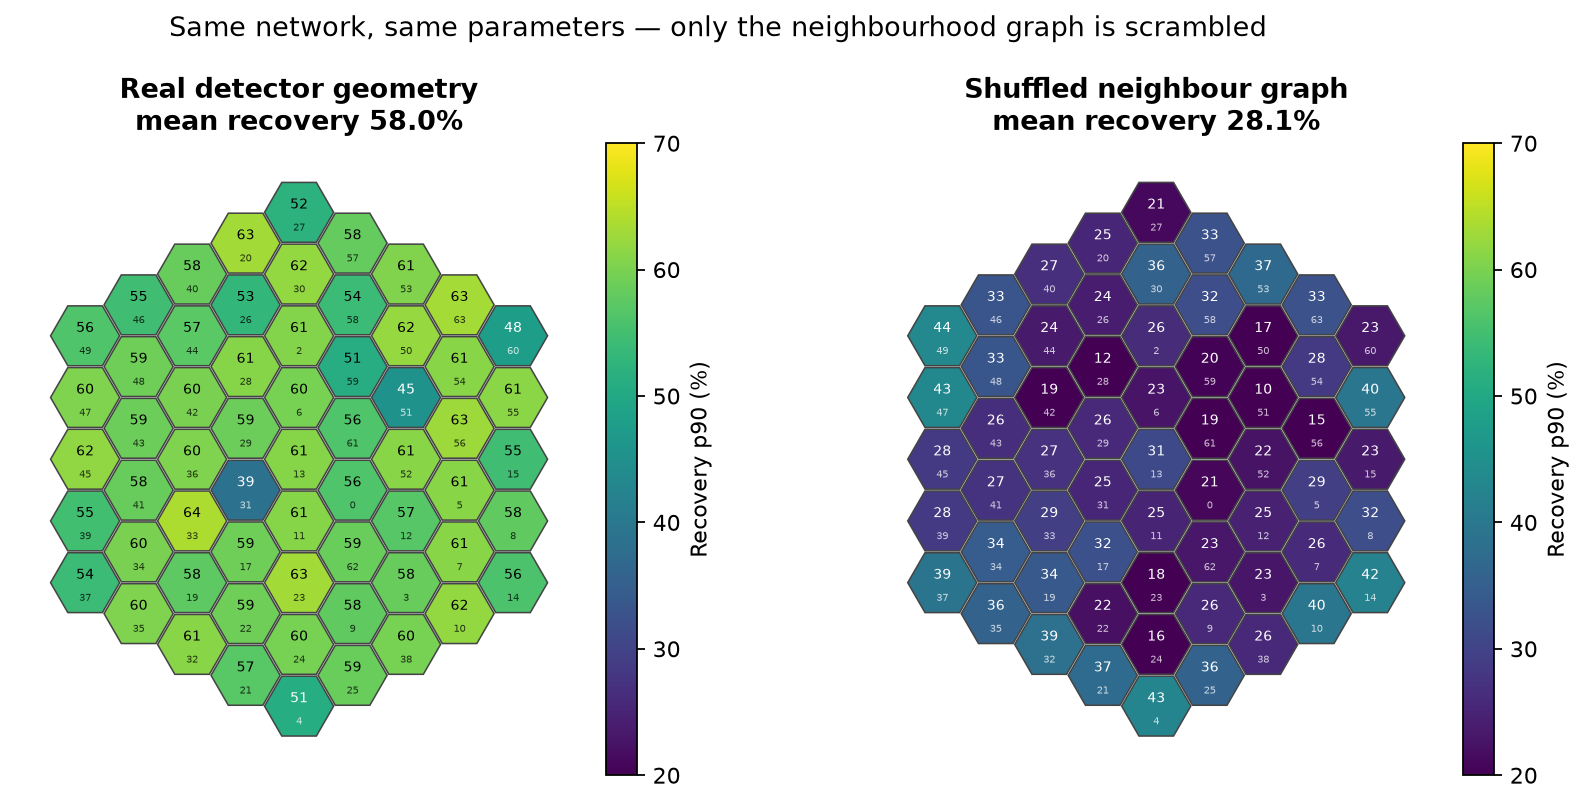
\includegraphics[width=\linewidth]{ablacion}
\caption{Effect of destroying the detector geometry. Recovery at the 90th
percentile for the reference model with the true adjacency and for three
independent random permutations of the graph that preserve node count, edge
count and degree distribution.}
\label{fig:ablacion}
\end{figure}

Against the classical methods, evaluated on the same channels, the network
recovers 57.9\,\% compared with 45.41\,\% for the neighbour mean and 46.56\,\%
for the per-channel linear regression, differences of 12.49 and 11.33
percentage points respectively.

We also quantified how far the useful information extends. Fitting linear
regressions restricted to concentric rings of neighbours gives 44.04\,\%
recovery with the first ring (5.1 channels on average), 46.42\,\% with the
second (13.7 channels) and 46.51\,\% with the third (24.1 channels), against
46.55\,\% when all 60 remaining channels are used.

\subsection{Reference Performance and Its Variability}

A single figure of merit says little without knowing how much it moves, so we
measured two sources of variability separately. Table~\ref{tab:reference}
reports both. Across four independent training runs, differing in the global
seed and in the module ordering, recovery at the 90th percentile is
$58.04 \pm 0.37$\,\% and the mean recovery is $52.15 \pm 0.31$\,\%.

\begin{table}[t]
\centering
\caption{Reference model and sources of variability. Values are mean $\pm$
standard deviation. $n$ is the number of independent runs.}
\label{tab:reference}
\begin{tabular}{@{}lccc@{}}
\toprule
\textbf{Source} & \textbf{$n$} & \textbf{Rec.\ p90} & \textbf{Rec.\ mean} \\
\midrule
Independent training runs & 4 & $58.04 \pm 0.37$ & $52.15 \pm 0.31$ \\
Data partition (CV)       & 5 & $56.56 \pm 2.32$ & $50.60 \pm 2.04$ \\
\bottomrule
\end{tabular}
\end{table}

However, repeating the split with five different partitions of the same 159
modules gives $56.56 \pm 2.32$\,\%, a standard deviation six times larger than
the one observed between training runs of a fixed partition. Measuring the
model on individual unseen modules makes the origin of that spread explicit:
recovery varies between 29.2\,\% and 63.0\,\% depending on the module, with a
standard deviation of 7.86 percentage points (Fig.~\ref{fig:variabilidad}),
which places the standard error of a mean over five test modules at 3.5 points.
The dominant uncertainty in this work is therefore which detectors happen to
fall in the test partition, not which weights the optimiser converged to.

\begin{figure}[t]
\centering
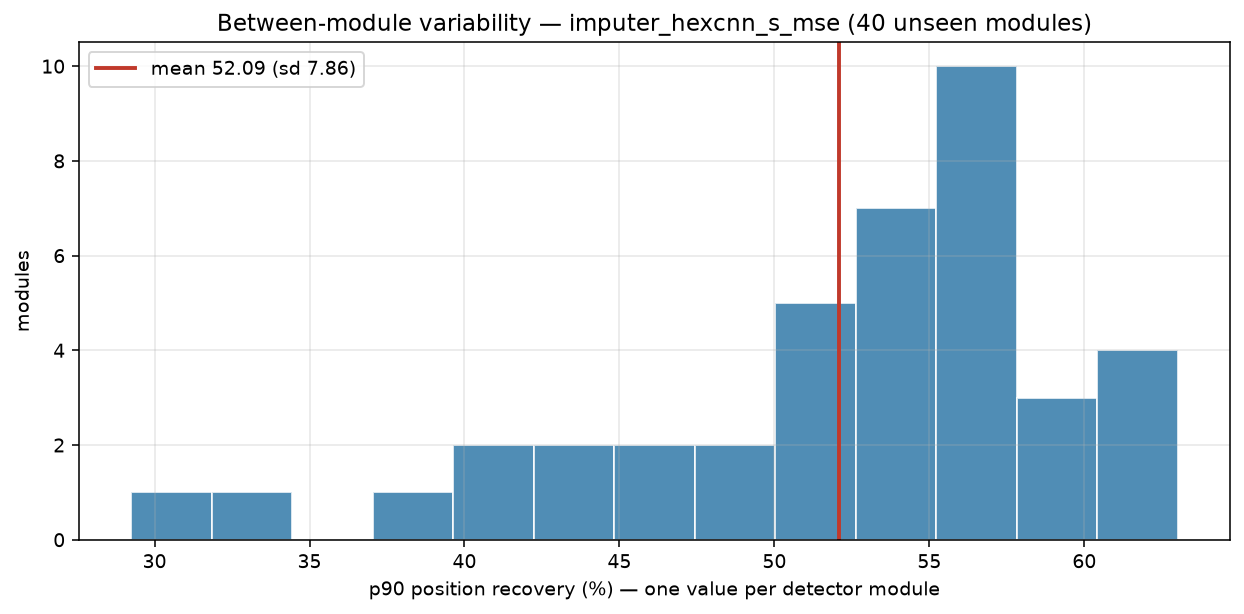
\includegraphics[width=\linewidth]{variabilidad_modulos}
\caption{Recovery at the 90th percentile measured on individual unseen
training modules. The spread between detectors (standard deviation of 7.86
percentage points) is an order of magnitude larger than the spread between
training runs on a fixed partition.}
\label{fig:variabilidad}
\end{figure}

Performance is not uniform across the detector.
Fig.~\ref{fig:mapa} maps the recovery of each of the 61 channels. The worst
channel of the reference band averages $42.29 \pm 4.45$\,\% over the four runs,
with individual values spanning 37.54\,\% to 47.76\,\%; the channel attaining
that minimum is not the same in every run, alternating between
$\mathrm{Ich}\ 60$ and $\mathrm{Ich}\ 31$.

\begin{figure*}[t]
\centering
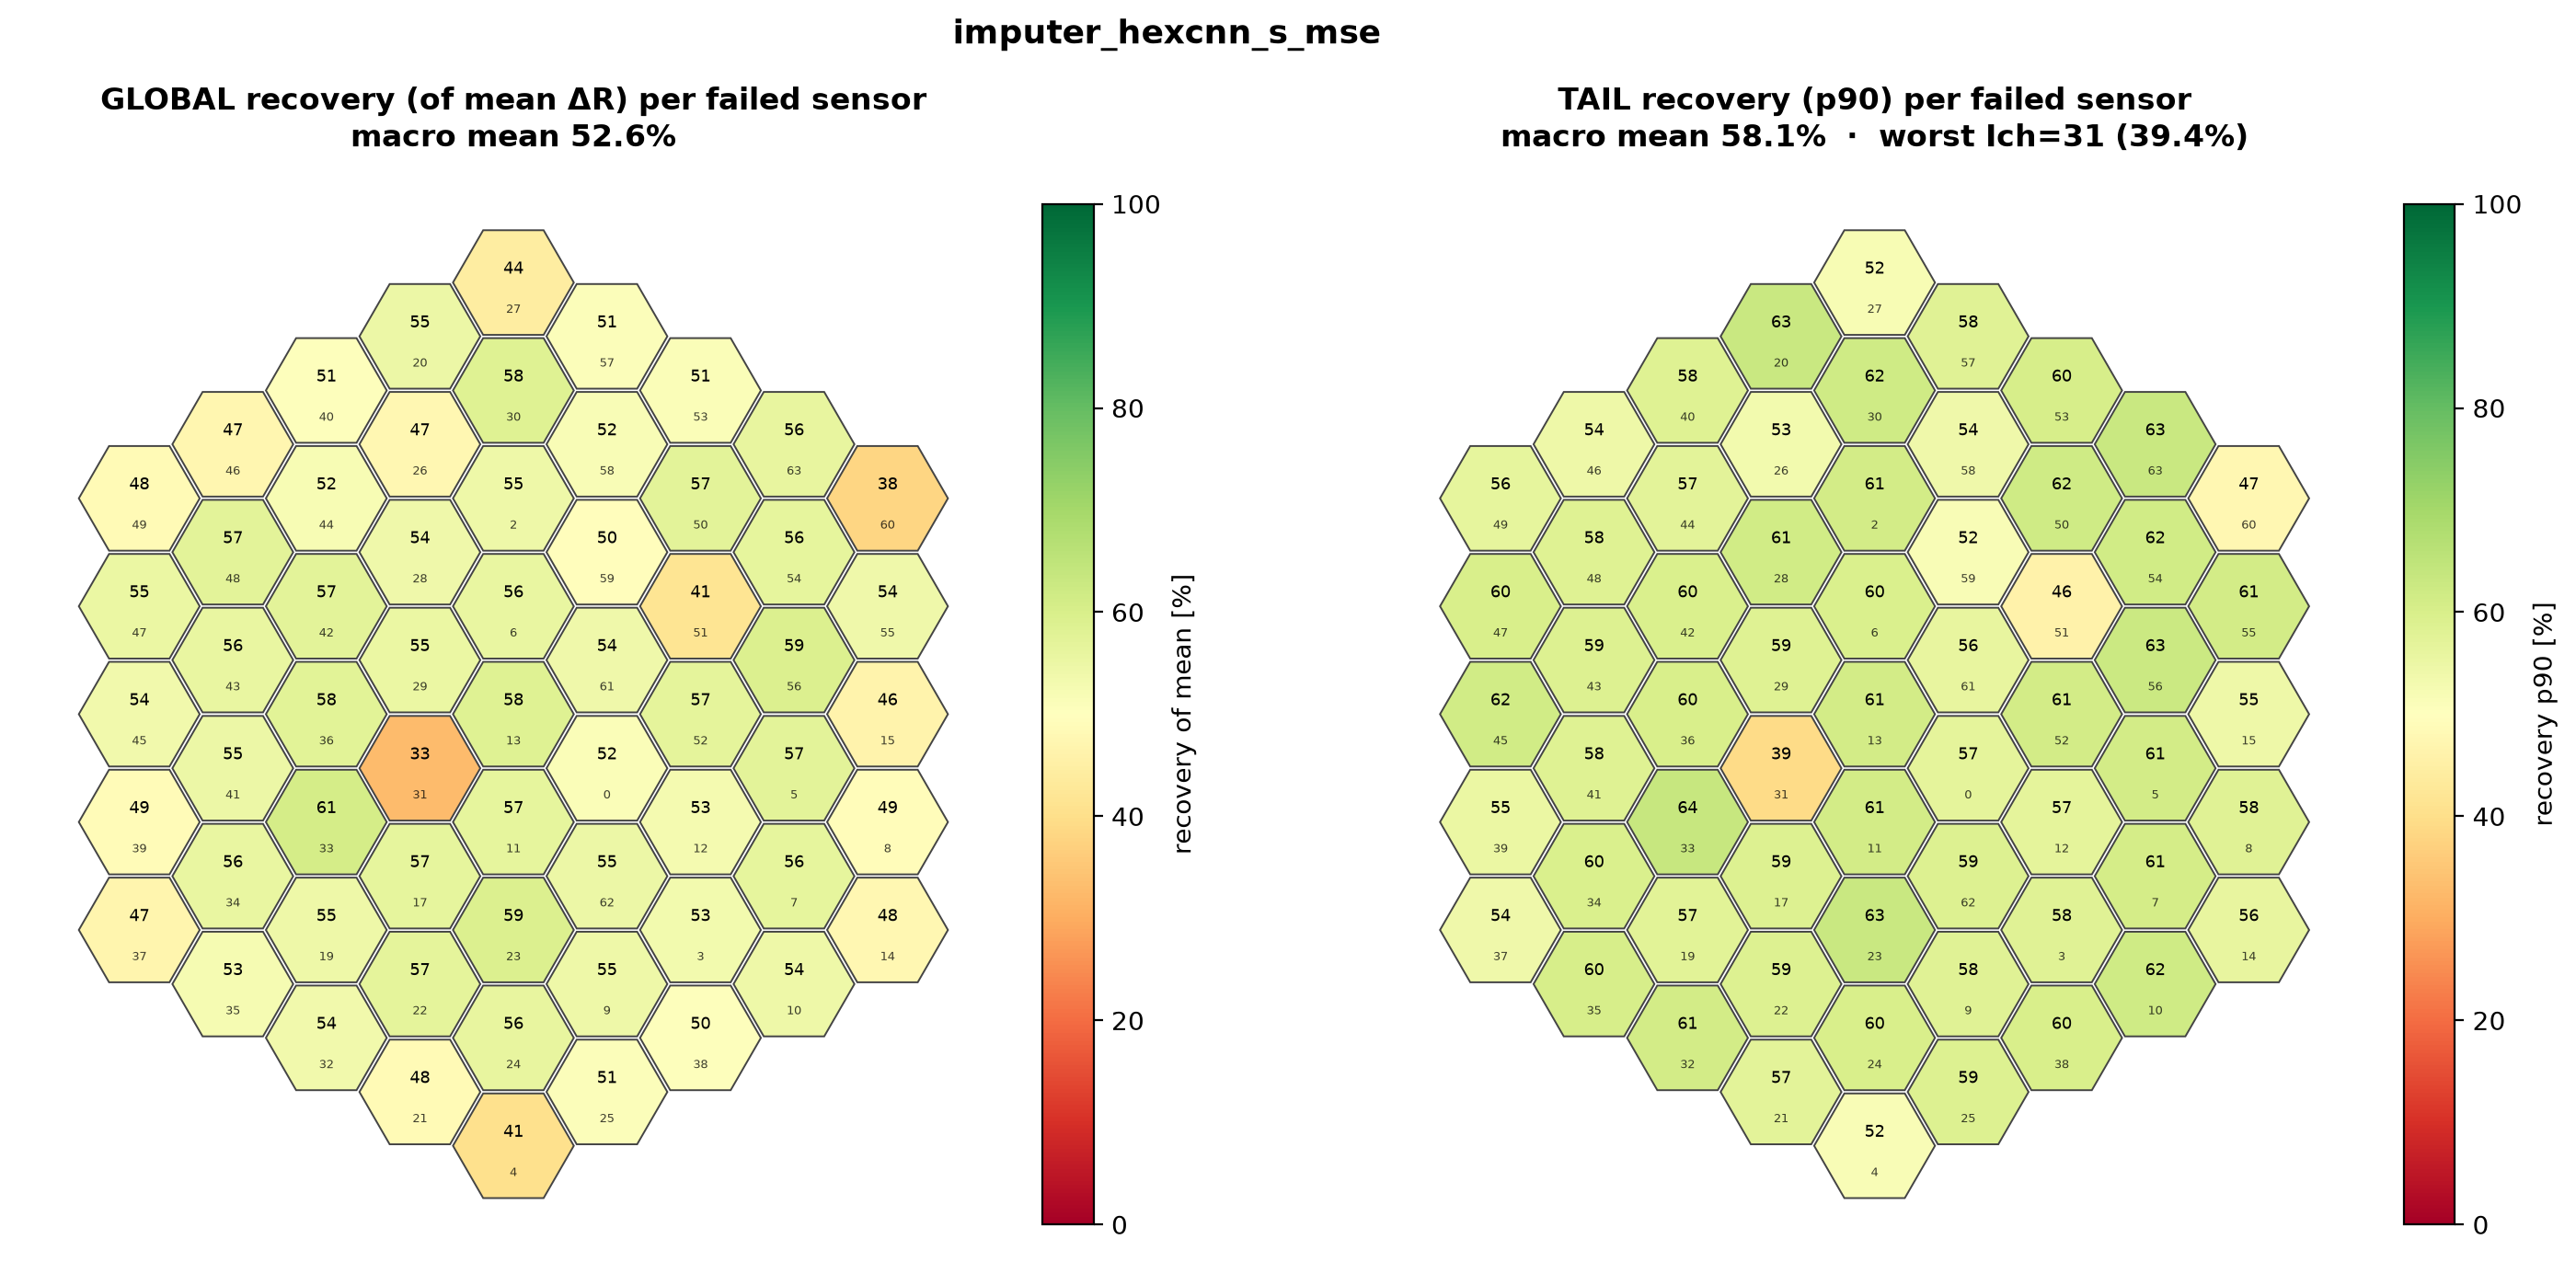
\includegraphics[width=0.86\textwidth]{mapa_recuperacion}
\caption{Per-channel recovery over the 61 active sensors. Left: recovery at the
90th percentile. Right: mean recovery. Channels at the perimeter of the
hexagonal array recover less charge than central ones.}
\label{fig:mapa}
\end{figure*}

The effect of imputation on the reconstructed image is shown in
Fig.~\ref{fig:floodmap}, which compares the flood map of a test module with one
channel suppressed against the same map after imputation.

\begin{figure*}[t]
\centering
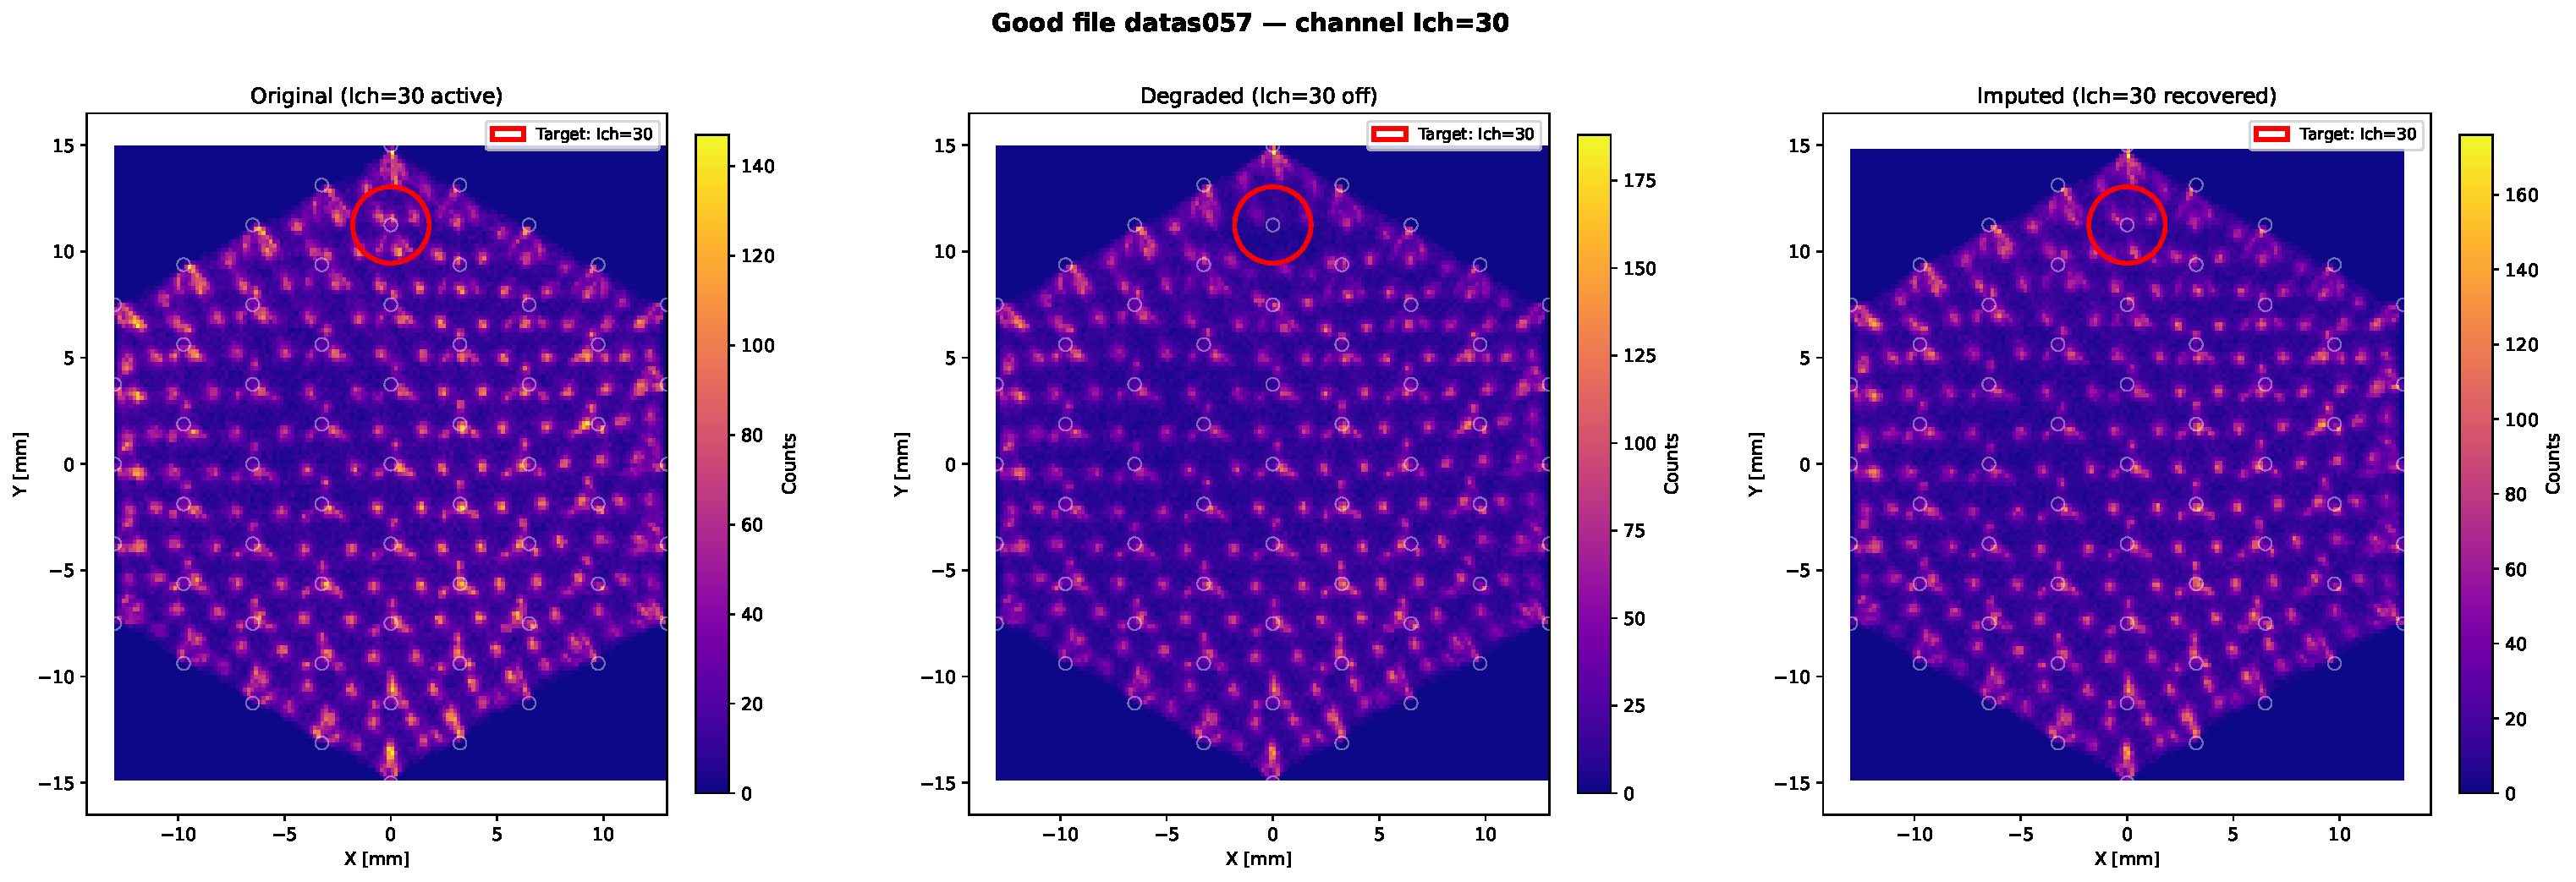
\includegraphics[width=0.86\textwidth]{floodmap}
\caption{Flood map of a test module. From left to right: reference map with all
channels active, map with one channel suppressed, and map recovered by the
model.}
\label{fig:floodmap}
\end{figure*}

\subsection{Multiple Simultaneous Failures}

Training with a single suppressed channel does not transfer to multiple
failures. Table~\ref{tab:multidead} reports recovery averaged over
$k = 1 \dots 4$ suppressed channels for the three spatial regimes. A model
trained with $k = 1$ falls to 33.74\,\% on contiguous failures, and its
standard deviation across runs rises to 11.68 points, since it performs
adequately at $k = 1$ and collapses at $k = 4$. Models trained with $k$ drawn
from 1 to 4 stay between 53\,\% and 58\,\% in all three regimes, with standard
deviations below 0.7 points.

\begin{table}[t]
\centering
\caption{Recovery at the 90th percentile by failure regime, averaged over
$k = 1 \dots 4$ suppressed channels. Campaign of 20 seeds and \num{200000}
events per file.}
\label{tab:multidead}
\begin{tabular}{@{}lccc@{}}
\toprule
\textbf{Training regime} & \textbf{Cluster} & \textbf{Near} & \textbf{Scatter} \\
\midrule
Single channel ($n{=}3$)
  & $33.74 \pm 11.68$ & $38.28 \pm 9.23$ & $47.69 \pm 4.95$ \\
Cluster, $k{=}1\!-\!4$ ($n{=}1$)
  & 58.46 & 52.62 & 52.44 \\
Near, $k{=}1\!-\!4$ ($n{=}3$)
  & $58.31 \pm 0.51$ & $54.61 \pm 0.58$ & $53.43 \pm 0.67$ \\
\bottomrule
\end{tabular}
\end{table}

Between the two multi-channel regimes, however, the differences are small. The
model trained on the \emph{near} regime exceeds the one trained on contiguous
clusters by 1.99 points in its own regime, a difference of 2.9 standard
deviations, while the two are indistinguishable on contiguous failures
($-0.14$ points) and on scattered ones ($+0.99$ points, 1.3 standard
deviations). Fig.~\ref{fig:regimenes} shows the three regimes side by side and
Fig.~\ref{fig:multidead} the degradation as $k$ grows.

\begin{figure}[t]
\centering
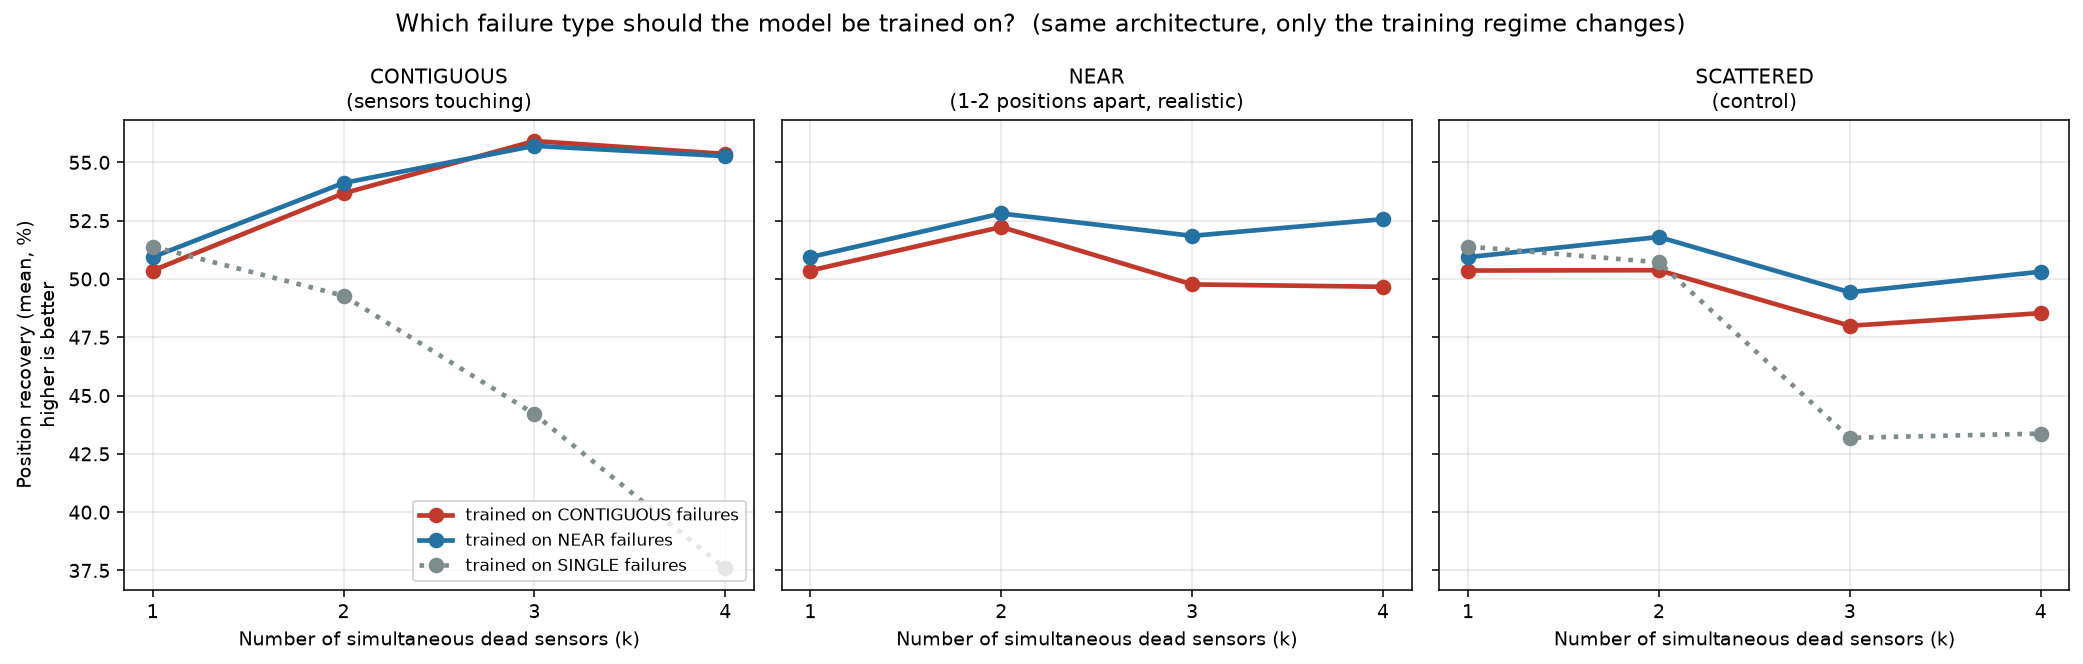
\includegraphics[width=\linewidth]{regimenes}
\caption{Recovery by failure regime for models trained under each of the three
mask-generation strategies.}
\label{fig:regimenes}
\end{figure}

\begin{figure}[t]
\centering
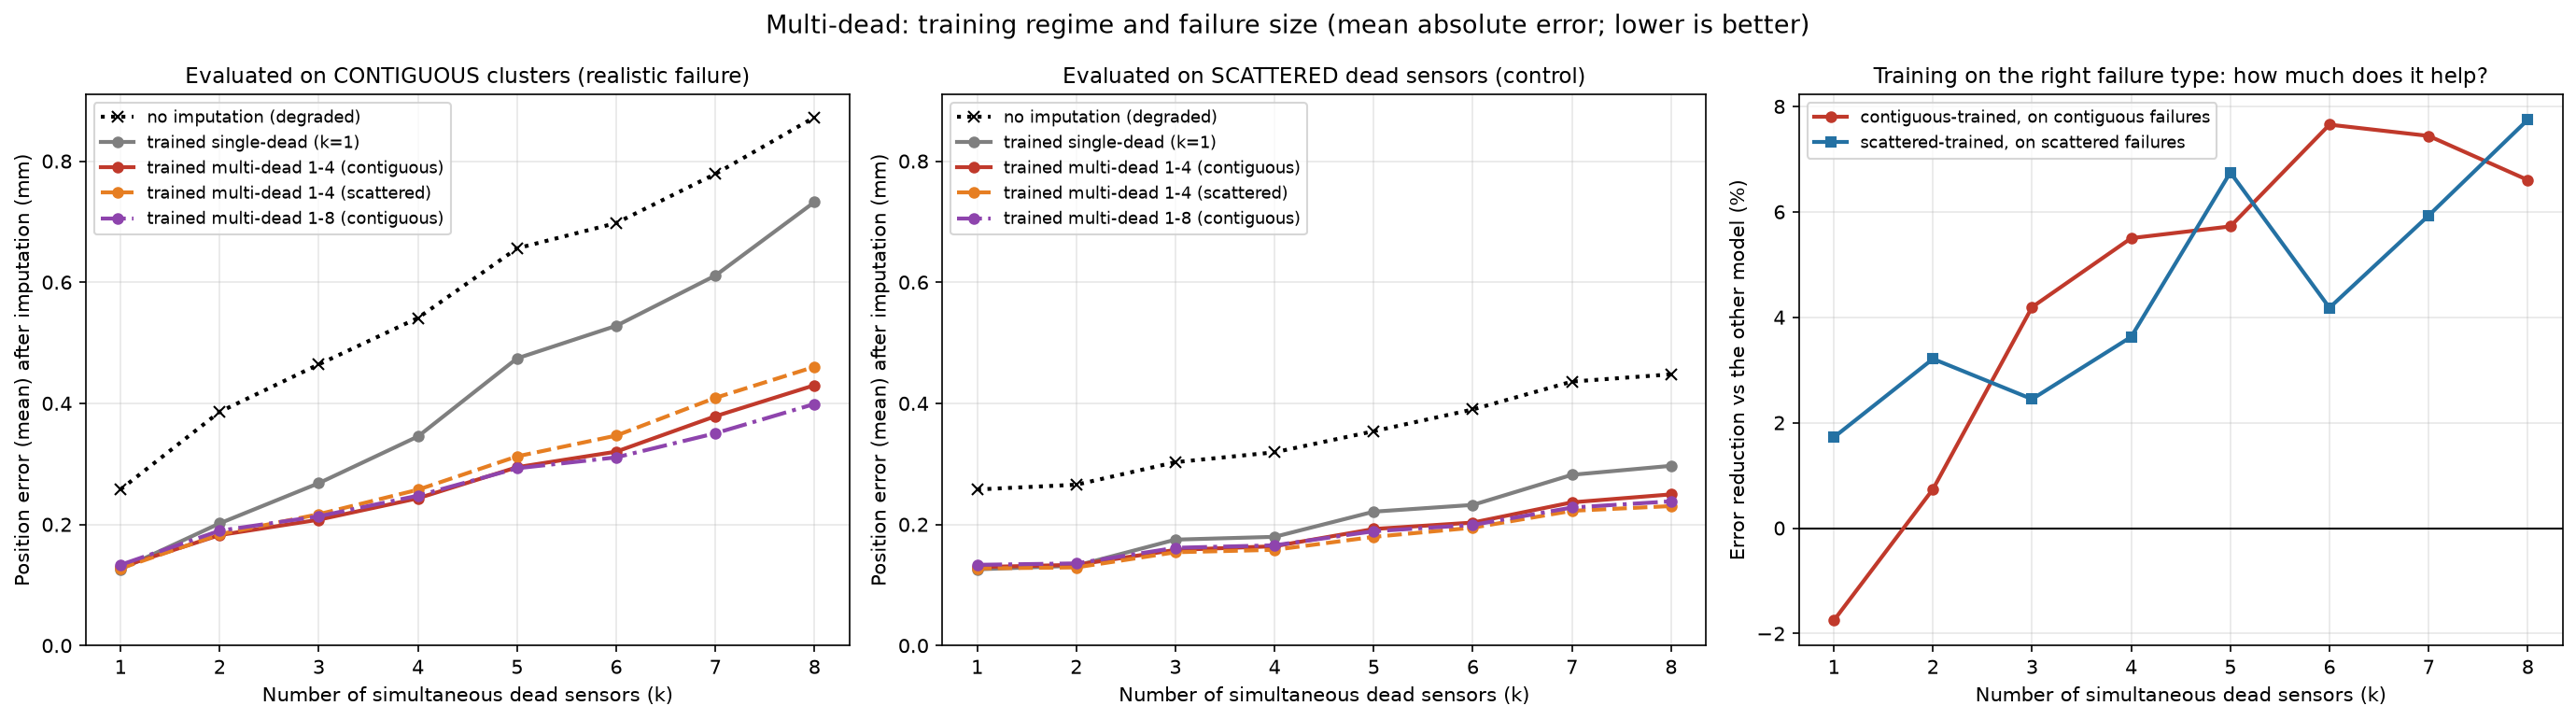
\includegraphics[width=\linewidth]{multidead}
\caption{Recovery as a function of the number of simultaneously suppressed
channels, for models trained with a single channel and with one to four.}
\label{fig:multidead}
\end{figure}

\subsection{Physical Fidelity}

Beyond the position error, we measured whether imputation preserves the two
physical quantities the detector is built to deliver.

The point-spread function of the flood map narrows from a macro-averaged FWHM
of 0.1656\,mm with a suppressed channel to 0.0847\,mm after imputation, a
recovery of 48.82\,\% of the induced blur (Fig.~\ref{fig:resolucion}). The
positional bias falls from 0.1262\,mm to 0.0218\,mm, a recovery of 82.71\,\%.

\begin{figure}[t]
\centering
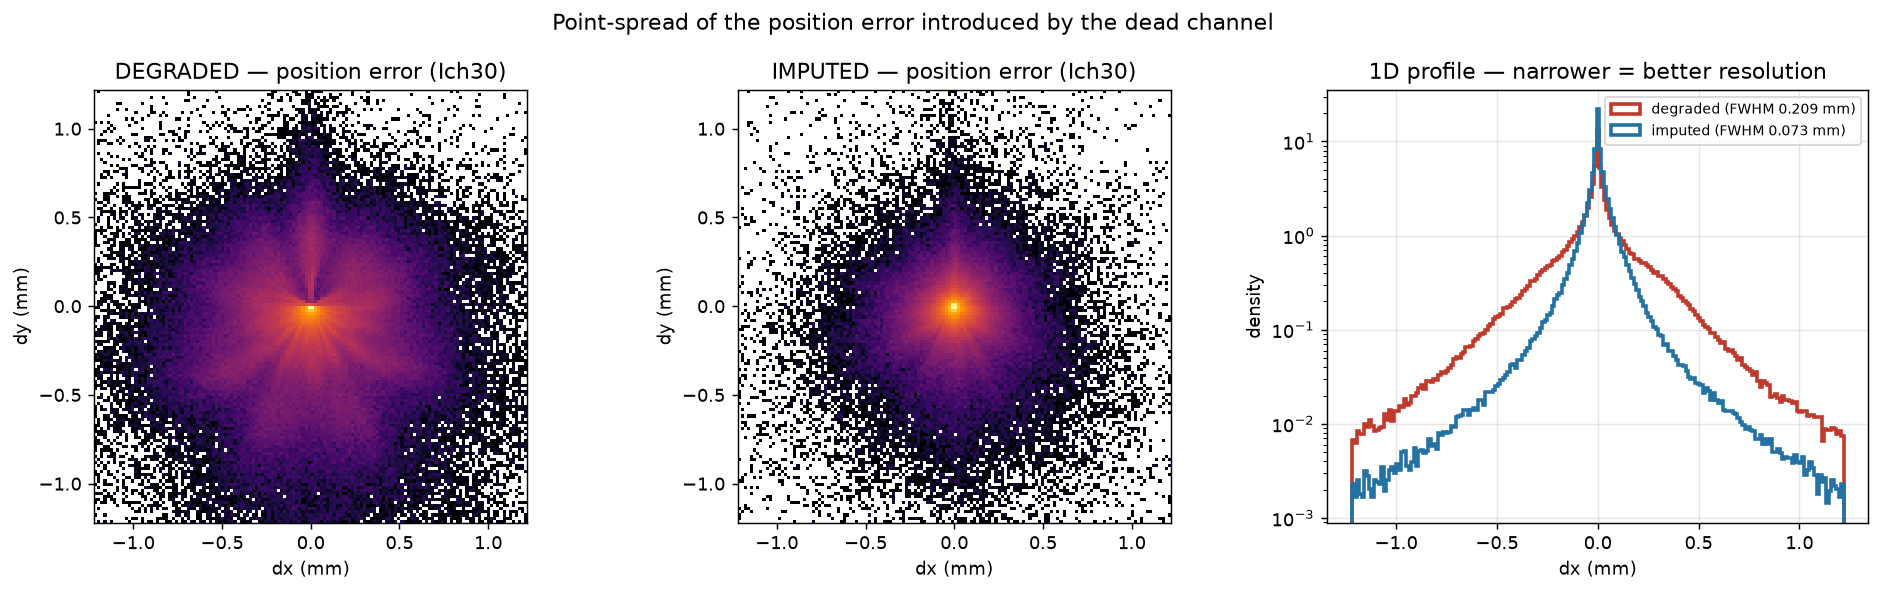
\includegraphics[width=\linewidth]{resolucion}
\caption{Point-spread function of the flood map with all channels active, with
one channel suppressed, and after imputation.}
\label{fig:resolucion}
\end{figure}

The energy spectrum is preserved to a comparable degree and with little
dependence on the region of the crystal: spectral recovery is 83.25\,\% in the
core, 84.32\,\% in the middle band and 81.19\,\% at the edge, for a global
value of 82.92\,\% (Fig.~\ref{fig:espectro}). The residual shift of the
photopeak stays between 0.20 and 0.24 ADC units across the three zones.

\begin{figure}[t]
\centering
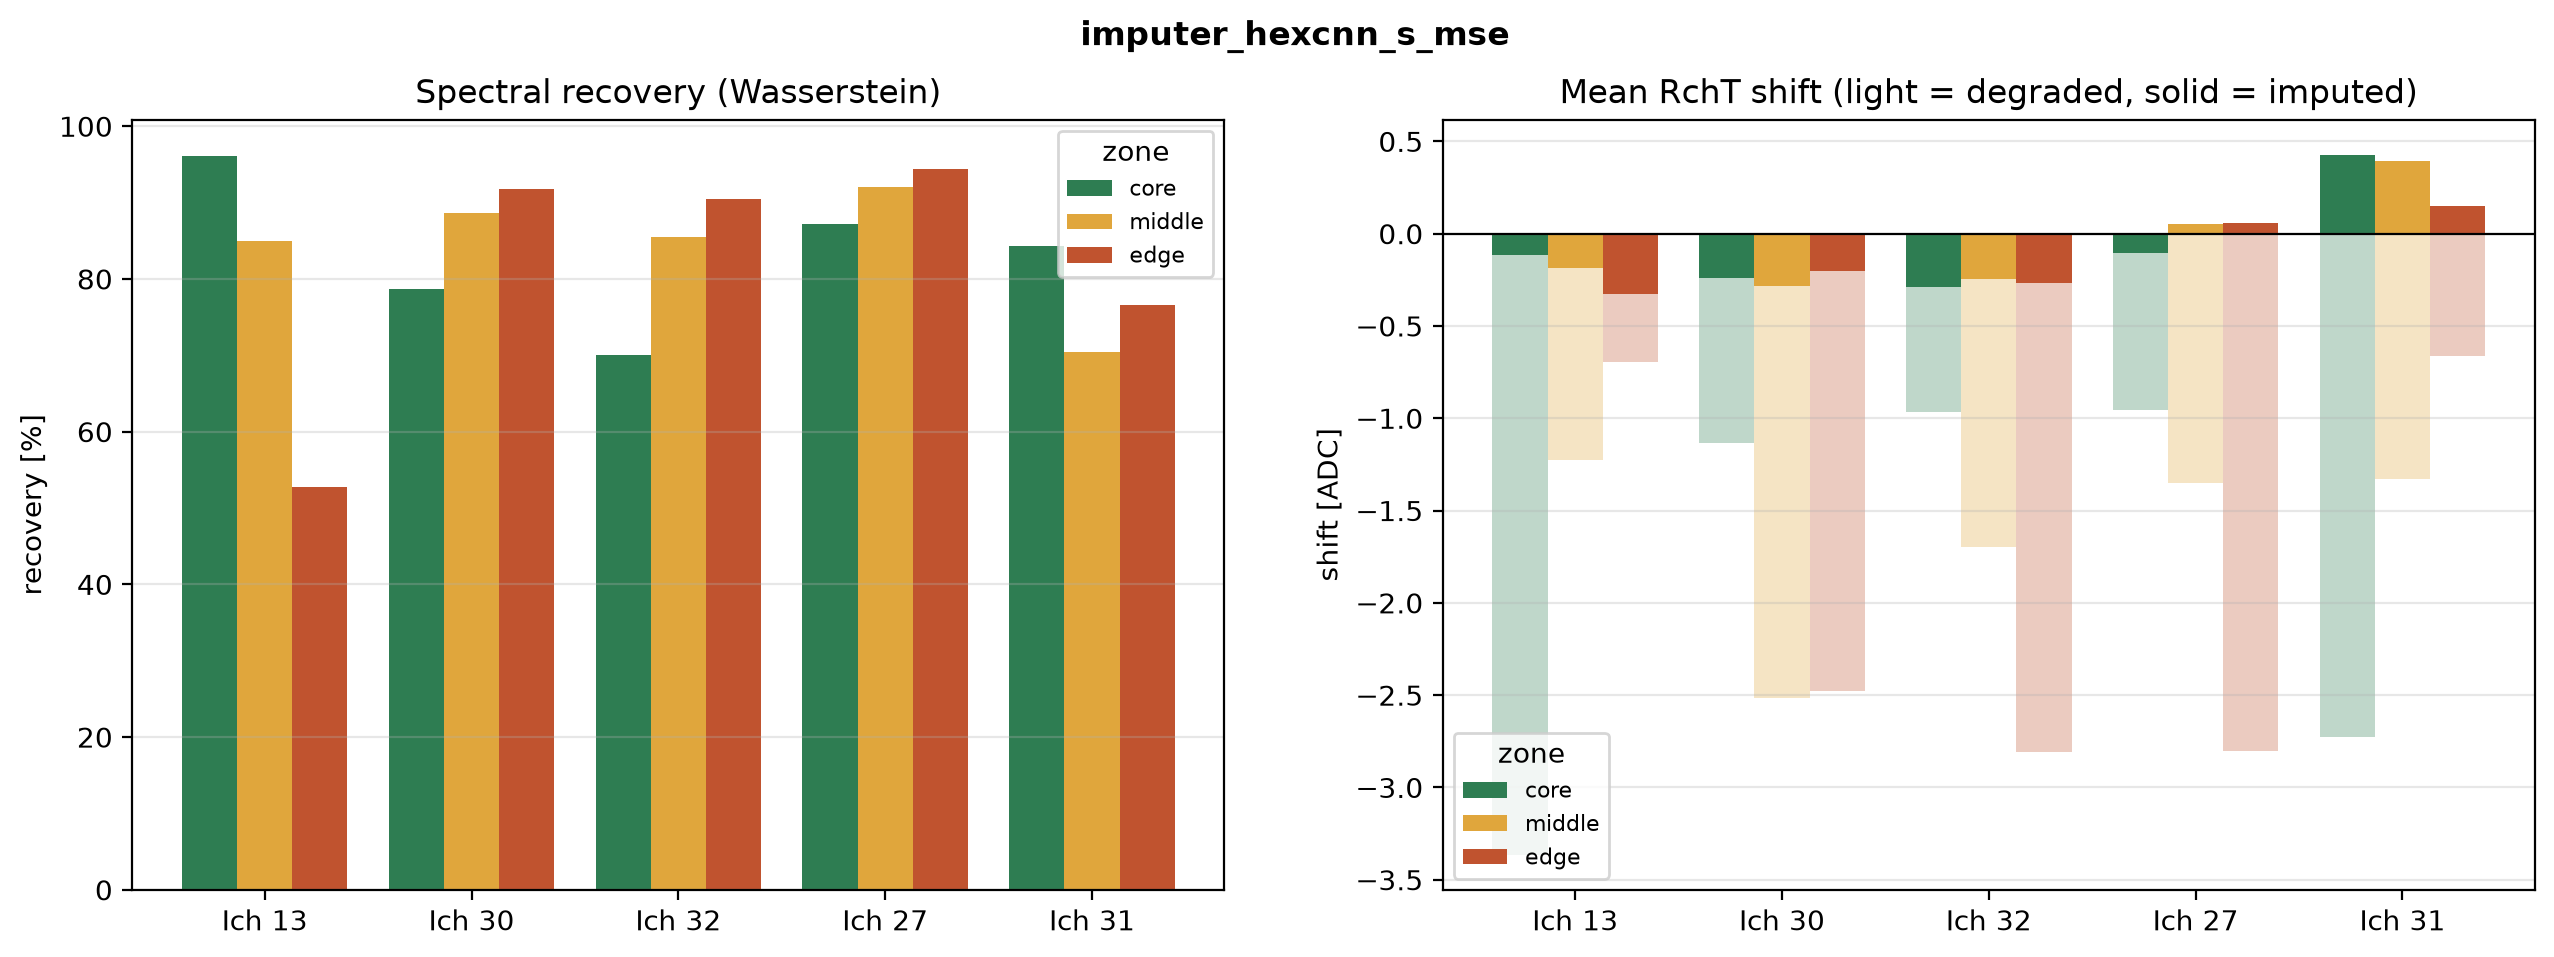
\includegraphics[width=\linewidth]{espectro}
\caption{Energy spectrum by crystal zone, comparing the original distribution
with the degraded and imputed ones. Zones are defined by concentric hexagonal
bands.}
\label{fig:espectro}
\end{figure}

\subsection{Physics-Informed Losses and Ensembles}

Adding the position error of Eq.~\ref{eq:centroid} to the loss leaves recovery
unchanged at 58.23\,\% against 58.02\,\% for the reference. Adding a term on
the energy spectrum degrades it to 46.04\,\%, with the bias changing sign.
Heteroscedastic prediction of mean and variance reaches 20.08\,\%.

Averaging the outputs of three independently trained replicas raises recovery
to 58.69\,\%, and averaging three different architectures raises it to
58.73\,\%, against $58.04 \pm 0.37$\,\% for a single model.

\subsection{Application to Faulty Modules}

On the \textsc{Bad} set, the detection statistic identifies fully dead channels
without error: the true positive rate is 1.00 for one, two, three and four
simultaneously suppressed channels when the injected severity is total
(Fig.~\ref{fig:roc}). Under partial degradation, in which the channel retains
70\,\% of its response, the rate falls to 0.95 for a single channel and 0.89
for two.

\begin{figure}[t]
\centering
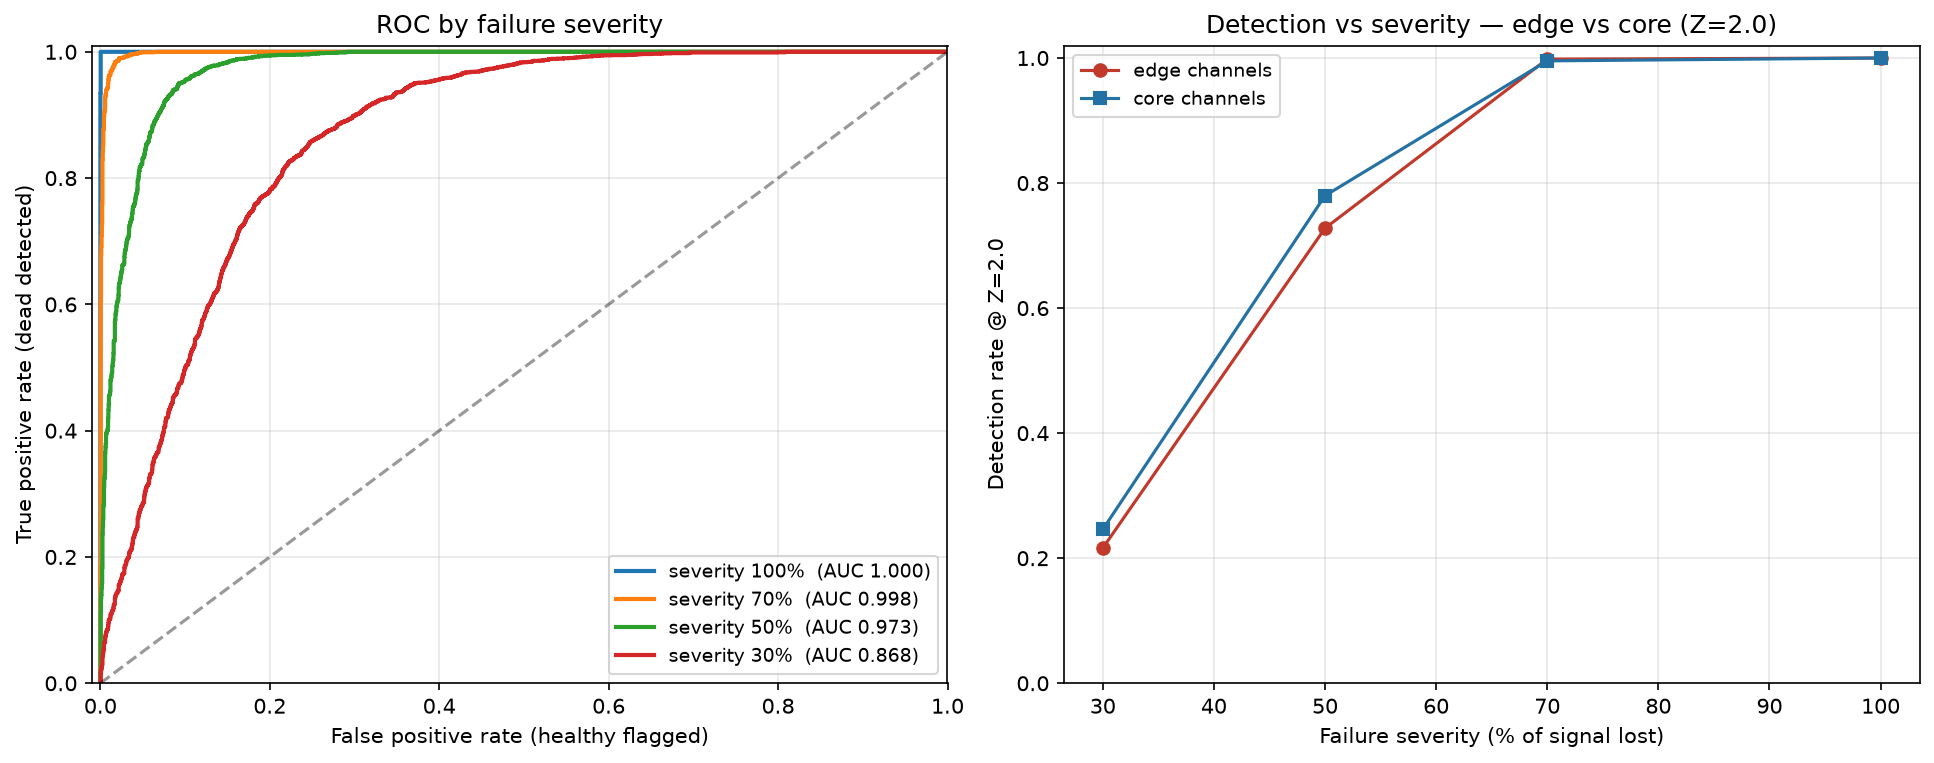
\includegraphics[width=\linewidth]{deteccion_roc}
\caption{Detection of faulty channels by ground-truth injection on healthy
modules. ROC curves for different numbers of simultaneously affected channels.}
\label{fig:roc}
\end{figure}

We labelled a subset of the \textsc{Bad} modules by visual inspection of their
flood maps to compare against expert criterion. At the time of writing, 18 of
the 62 modules have been annotated, yielding 29 channels marked as faulty
across 14 modules; the remaining 4 modules were judged to have no defective
channel.
% TODO(dato): completar el etiquetado de los 62 modulos y calcular el acuerdo
% experto-vs-estadistico sobre el conjunto completo.


% ---------------------------------------------------------------------
\section{Discussion}
% ---------------------------------------------------------------------

Interpretacion, comparacion con el estado del arte y limitaciones.


% ---------------------------------------------------------------------
\section{Conclusions}
% ---------------------------------------------------------------------

Conclusiones y lineas futuras.


% ---------------------------------------------------------------------
% REFERENCIAS
% ---------------------------------------------------------------------
\bibliographystyle{IEEEtran}
\bibliography{referencias}

\end{document}